\chapter{Implementation}\label{chap:implementation}
This chapter is dedicated to the description of the re-implementation of several existing models, along with our modifications, and the implementation details of the novel proposed method. We will introduce the architecture of the models, as well as the data pre-processing, training procedures and optimization parameters used.

\section{Re-implementation of existing models}

\subsection{Deep Depth Pose model}
In this section, we are going to describe our re-implementation of the DDP model (proposed in~\cite{Marin18jvcir}) in Keras framework. The follow-up additional modifications of the model, which are presented at the end of the section.\par
\vspace{5mm}
\noindent
The DDP model is based on the idea of linearly combining the predefined prototype poses to obtain the resulting pose estimation. The set of prototype poses is produced by clustering the training dataset into $K$ clusters, $K$ being a hyperparameter of the network. The output of the model represents $K$ weights, each corresponding to one of the prototype poses. The final estimated pose is then obtained as a sum of the weighted prototypes.


\subsubsection{Model structure}

The architecure of the DDP model itself is relatively simple. The model is actually not very deep, it consists of five convolutional blocks, each followed by ReLU activation. First three blocks also contain a pooling layer, as indicated in Figure~\ref{fig:ddp}. After the convolutional blocks, there are three fully-connected layers. The number of neurons in the output layer is a hyperparameter set to the number of prototype poses clustered from the dataset. The input to the model is a one-channel depth map of size 100 x 100 pixels.\par

\vspace{5mm}
\begin{figure}[H]
\begin{center}
  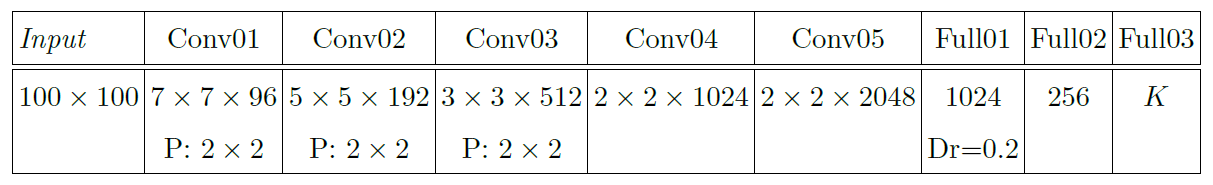
\includegraphics[width=\textwidth]{images/implementation/ddp.PNG}
  \caption[Deep Depth Pose model architecture.]{Deep Depth Pose model architecture~\cite{Marin18jvcir} (\textit{P} stands for pooling layer, \textit{Dr} indicates dropout, $K$ is the number of prototype poses).}
  \label{fig:ddp}
\end{center}
\end{figure}


\subsubsection{Loss function}

The loss function used during training the model is defined as huber loss with a regularization term, as described in Equation~\ref{eq:huberloss}, where $\mathcal{L}_R$ is the (residual) huber loss.\par

\begin{equation}
\mathcal{L}_{DDP}(g(\mathbf{D}, \theta), \mathbf{C}, \mathbf{p}, \alpha) = (1 - \alpha) \cdot \mathcal{L}_R(\mathbf{C} \times g(\mathbf{D}, \theta), \mathbf{p}) + \alpha \cdot \|g(\mathbf{D}, \theta)\|_1 \label{eq:huberloss}
\end{equation} 

\noindent In the equation above, $g(\mathbf{D}, \theta)$ represents a non-linear function computed by the neural model on the input depth map $\mathbf{D}$ with trainable parameters $\theta$, returning a column vector of length $K$ (number of clustered prototype poses), $\mathbf{C}$ is a matrix with $K$ columns containing prototype poses, $\mathbf{p}$ stands for the vectorized ground truth pose,  and $\alpha$ is a regularization coefficient  – a hyperparameter to control the magnitude of the resulting weights of the prototypes.

\subsubsection{Initialization}

The values of the model's hyperparameters from the original DDP paper were chosen using the 'Mann-Whitney U-test'~\cite{mann1947}, thus determining, whether the median difference between pairs of configurations are statistically significant. The value of the regularization coefficient was fixed to $\alpha = 0.08$ for the ITOP dataset, and $\alpha = 0.01$ for the UBC3V dataset. The number of prototypes was set to $K=70$ and $K=100$ regarding the ITOP and the UBC3V dataset respectively.\par
\vspace{5mm}
\noindent
The model learns using the Adam optimizer with the learning rate set to $10^{-3}$, which is progressively decreasing during the training.  The weights in the model are initialized using the Xavier normal initializer, that is randomly chosen from the normal distribution with zero mean and a standard deviation proportional to the filter size. The biases are initially set to zero. The size of batches is set to $b=64$.

\subsubsection{Data pre-processing}

In the pre-processing stage, the depth maps are re-sized to match the model input dimensions. First, the image is cropped along the larger dimension on both sides to fit the square, assuming the subject is located near the center of the image. Then, the image is re-sized to $100\times100$ px. Afterwards, the depth values are normalized to range [0,1]. Also, the input depth images are normalized globally by subtracting the mean image of the training set from each depth sample. The ground truth poses are being normalized as well – to zero mean and one standard deviation.\par
\vspace{5mm}
\noindent 
Concerning the datasets used for evaluation, UBC3V already comes with the split into the train, validation and test set. The ITOP dataset is originally divided into the train and test set only, thus the validation set was acquired by random sampling of the train data. The ratio was set to 80/20, meaning the data used for validation are representing 20\% of the train set. During the experiments, only the hard-pose part of UBC3V, and the side-view part (for single-view approach) of the ITOP dataset were used.

%\subsection{Train phase}
%
%\subsection{Test phase}

\subsubsection{Modifications}
This section introduces several modifications we have made to the proposed DDP model, in order to lower the mean error of the predictions. Since the experience of the researchers made us believe that the implementation of the same model in different framework often leads to different results, we diverted from the original architecture of the model, as well as the initial optimization parameters.\par
\vspace{5mm}

\noindent
However, still inspired by the DDP model, we have built a slightly deeper, more complex model, in an attempt to improve the final estimations, assuming the original architecture was not able to fully retain the complexity of the specified task. We used both ITOP and UBC3V datasets again, for the evaluation of the modified model.
The architecture of the modified DDP network is shown in Figure~\ref{fig:mddp}. As shown in the figure, we significantly increased the amount of dropout layers, as the model tended to overfit the training data. Moreover, two additional convolutional layers were stacked in the model architecture, to enhance the nonlinearity of the network (introduced by the ReLU activations used after convolutions).\par
\vspace{5mm}

\begin{figure}[H]
\begin{center}
  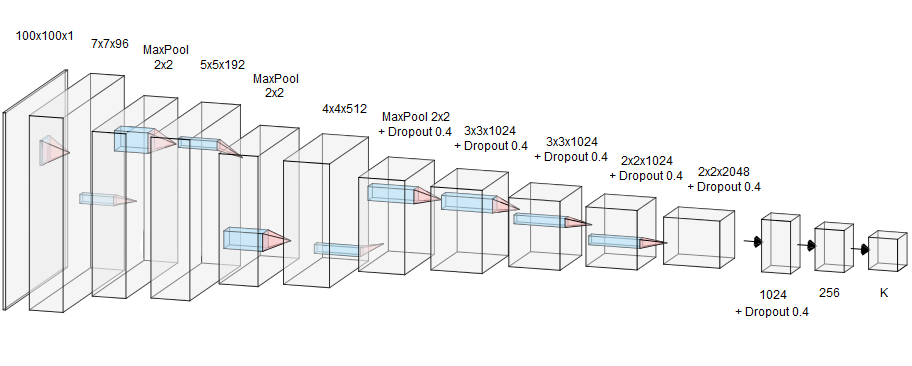
\includegraphics[width=\textwidth]{images/implementation/mddp.png}
  \caption[Our modification of the original DDP model architecture.]{Our modification of the original DDP model architecture\break (\textit{K} stands for the number of prototype poses).}
  \label{fig:mddp}
\end{center}
\end{figure}


\noindent Besides the structure of the model, some of the hyperparameters were slightly modified as well, mainly due to switching to another deep learning framework, where the back-end procedures differ, which may be resulting in a convergence to different outputs. Based on the experiments, the regularization parameter was fixed to $\alpha = 0.1$ for both benchmark datasets. The residual huber loss has been replaced by an absolute error, and the L2 norm was used in the regularization term instead of the L1 norm. Even though in the original paper, the authors indicate the L1 norm is more robust to outliers, our tests in the utilized framework led to a conclusion, that using the L2 norm as a regularization term in the loss function was more helpful to the loss minimization. Also, the initial learning rate was reduced to $10^{-4}$, due to an occasional undesirable divergent behavior of the model loss.\par
\vspace{5mm}
\noindent Regarding the test phase, the experiments on the ITOP dataset have shown that even though the test set seems sufficiently representative (that is, retains the approximate distribution of the training set), the error on the test data is by far worse than the error on previously unseen data obtained by random sampling of the training set (used as a validation set). This is probably caused by the fact, that the input data is formed by a sequence of video frames, thus many subsequent samples captures almost the same content, with only a minimal shift between the frames. As a result, a lot of the validation samples are nearly the same as the ones used for training.\par
\vspace{5mm}
\noindent
The final results of both the original DDP and modified DDP model, evaluated on the test set of ITOP and UBC3V datasets, are reported and discussed in Chapter 7.


\subsection{Point-Based Pose Estimation model}

As another part of our study, we chose to examine the Point-Base Pose Estimation (PBPE) model introduced in~\cite{Ali19}. Again, we re-implement the method in Keras framework, and propose further modifications of the model at the end of the section.\par
\vspace{5mm}
\noindent % TODO este popisat zakladnu myslienku modelu
The model is heavily inspired by the implementation of PointNet~\cite{DBLP:journals/corr/QiSMG16}, which was built for the task of object classification and semantic segmentation. Basically, the architecture has been modified to fit the task of human pose estimation, making use of the auxiliary sub-network contributing to the global model loss.


\subsubsection{Model structure}
The architecture of the proposed model consists of two branches (or sub-networks). The auxiliary sub-network is included to compute the body part segmentation on the fly, while the main network regresses the joint locations. The basic idea behind the structure of the model is the aggregation of both local and global features of the input point cloud in the auxiliary part-segmentation network. Without the sub-network, almost all of the local context would be lost because of the max-pooling operation in the intermediate layers. The incorporation of the local features helps the network understand the relationships among particular local regions of the human body. The whole architecture of the stated model is shown in Figure~\ref{fig:PBPE}.\par
\vspace{5mm}

\begin{figure}[H]
\begin{center}
  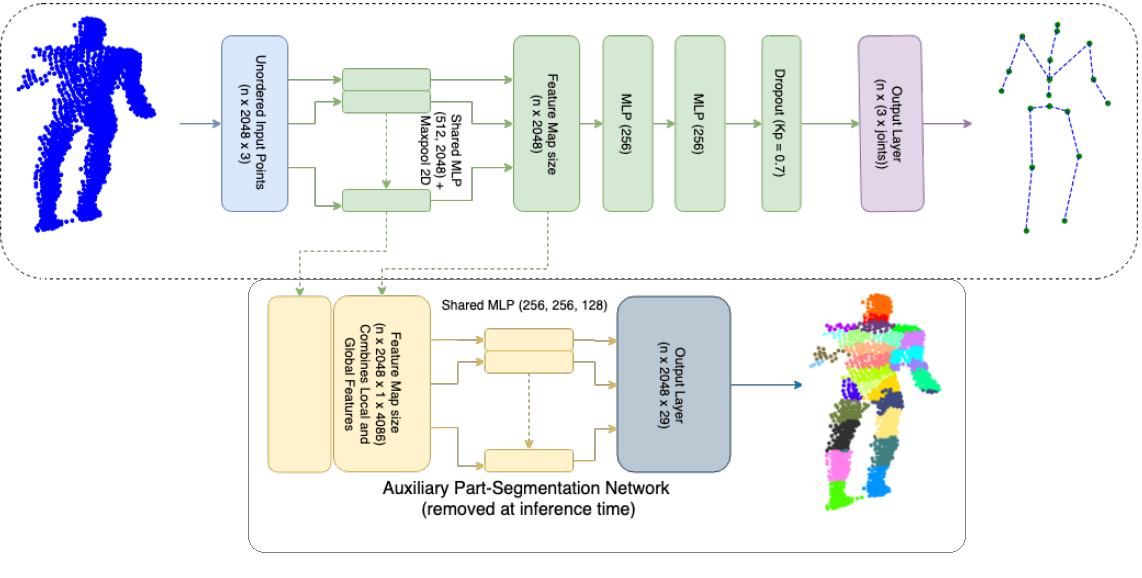
\includegraphics[height=200px]{images/implementation/pbpe2.PNG}
  \caption[The Point-Based Pose Estimation model architecture.]{The Point-Based Pose Estimation model architecture~\cite{Ali19}.}
  \label{fig:PBPE}
\end{center}
\end{figure}

\noindent
As already mentioned, the unorganized and irregular depth input represented by a point cloud is a key factor in this architecture. For this very reason, the engagement of the classic convolution operation is not possible, since the point cloud provides no explicit spatial information about the neighboring points. In this case, pseudo-convolutions with a kernel size of $1\times1$ are employed. The functionality of such pseudo-convolution layers lies in reducing (or expanding) the dimensionality in the filter space. Shared multi-layer perceptron (shared MLP) stands for a stack of the $1 \times 1$ convolution layers, each followed by batch normalization and ReLU activation, as illustrated in Figure~\ref{fig:PBPE}. The numbers in the parentheses indicate the number of filters in particular layers.\par
\vspace{5mm}
\noindent After the shared MLP, the regression branch consists of two fully-connected layers and an output layer. Each dense layer is also followed by a batch normalization layer and ReLU activation. The input of the model is of shape $(b \times p \times 3)$, where $b$ represents the batch size, and $p$ is the number of points in the input point cloud, each located by three coordinates. The output shape of both sub-networks depends on the number of joints in the skeleton structure. The number of joints, as well as the number of points the point clouds are containing, is a hyper-parameter.\par
\vspace{5mm}
\noindent The input passed to the auxiliary segmentation sub-network is formed by concatenating the local and the global features obtained in the regression branch. The local features contains the outputs of pseudo-convolutions before the max-pooling is applied. The global features are acquired as the result of max-pooling across all points in the point cloud. The auxiliary sub-network outputs per-point labels segmenting the input point cloud into particular body parts.\par
\vspace{5mm}
\noindent One of the conveniences of the PBPE model is the optional omission of the auxiliary branch at test time. Since we are focusing strictly on the task of pose estimation, the body part segmentation is only relevant for us in a context of training (and contributing to the model loss). Hence, we can prevent the data from being passed through the segmentation branch at the inference time, saving computational cost and time.

\subsubsection{Loss function}
As a loss function of the regression branch, the model uses a simple mean squared error. Regarding the segmentation branch, the categorical cross-entropy is being used, since it is essentially a classfication task.\par
\vspace{5mm}
\noindent
According to our experiments, without the segmentation sub-network, the model tends to slightly overfit the train data. The loss of the auxiliary segmentation branch is contributing to the global loss to help the model generalize better on previously unseen data. Originally, the weight of the contribution was set to $w_a=0.1$. The default weight of the global loss is $w_g = 0.9$. 


\subsubsection{Initialization} 
The weights inside the model are sampled from the normal distribution with zero mean and standard deviation relative to filter size, using the Xavier initializer. Following the PBPE proposal, the initial learning rate is set to $10^{-3}$, and is reduced exponentially with a decay rate $d = 0.5$ in each epoch. Also, the learning rate is clipped at the value of $10^-5$, in order to prevent the model training from getting stuck in local minima. The model is trained using the Adam optimizer. In each step, the model processes a batch of size $b=32$.\par
\vspace{5mm}
\noindent Another essential hyper-parameter is the predefined number of points in the input point clouds. The value is set to $p=2048$, which seems to be an adequate amount of points to cover the whole human pose with enough complexity. Therefore, every point cloud needs to be sub-sampled to this number of points, prior to feeding it to the network. The number of joints in the skeleton representation, defining the output shape of the both model branches, should be adjusted according to the dataset the network is processing at the moment.

\subsubsection{Data pre-processing}
Depending on the single or multi-view approach, the input point clouds are treated each as a single sample, or the different viewpoints of the same frame are merged into a single point cloud. Based on the existing studies, inference from multi-view input data is expected to give more accurate results, however the single-view based estimation is far more useful in most of the real-time applications, since there is no need for camera synchronization. Therefore, we have carried out experiments inferring from multi-view, as well as single-view input data.\par
\par
\vspace{5mm}
\noindent
As the next pre-processing step, the point clouds were sub-sampled to the specified number of points ($p = 2048$) using the farthest point sampling technique. The input point clouds and the corresponding joint locations were normalized to the range $ [-1, 1]$ using the minimum and maximum values of the whole training set. Concerning the validation and test data, there were two options, how to normalize them – either using the scaling parameters of the training set, or scale the validation and test set to the specified range with its own parameters. However, since the model is designed to work in a scenario, where the test data are fed into the network one-by-one, the only possible option is scaling it using the known parameters of the train set.\par

\vspace{5mm}

\begin{figure}[H]
\begin{center}
  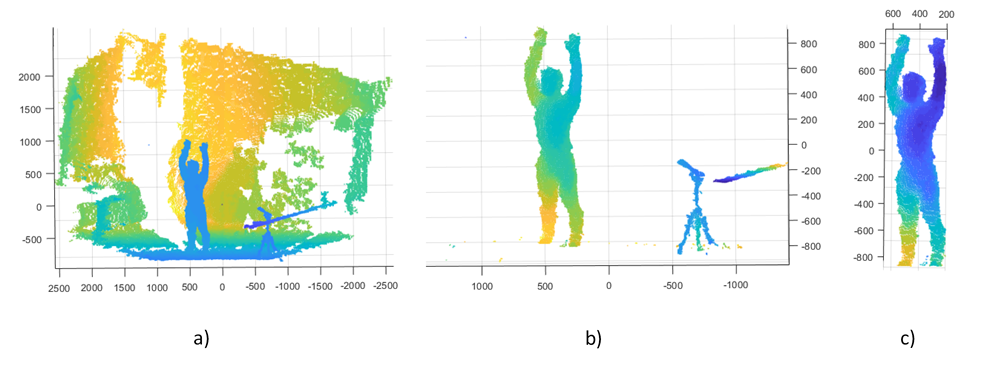
\includegraphics[width=\textwidth]{images/implementation/mhad.png}
  \caption[Data pre-processing shown on a sample point cloud from MHAD dataset.]{ Data pre-processing shown on a sample point cloud from MHAD dataset a) before segmentation, b) after removing the background and floor, c) after final clustering.}
  \label{fig:mhad}
\end{center}
\end{figure}

\noindent
Since the used datasets (except for the UBC3V) captures real-world data, the raw point clouds contain a lot of noise. Therefore, we consider suitable preprocessing as a very important step. First, the background wall and the floor are removed by MSAC plane fitting (which is a variation of RANSAC algorithm). Then, the segmentation of the point cloud into clusters based on Euclidean distance is performed, and the biggest cluster is considered as the desired subject. Figure~\ref{fig:mhad} depicts a sample from MHAD dataset, before and after applying the segmentation pipeline.% TODO spoliehame sa pri clusterovani na to, ze ludsky subjekt je v obraze najvacsi, teda nenachadzaju sa v scene ine objekty, vacsie ako actor.
\par

\vspace{5mm}
\noindent
The MHAD dataset does not provide any partition into the train and test data. Thus, we carried out experiments using two different protocols: (a) choosing the test set as randomly sampled $25 \%$ of the dataset, (b) leave-one-subject-out cross validation. As already pointed out in the original proposal of the PBPE model, the skeleton representation in the MHAD dataset is very detailed, yielding a total of 35 skeletal joints. We have slightly modified the original skeleton structure by removing several redundant joints – one pair repeated at fingertips, two additional pairs present at toe tips. This way, we restricted the skeleton to the resulting 29 joints (as shown in Figure~\ref{fig:mhad_skeletons}), in the same way as in~\cite{Ali19}. However, we present results of our approach also on the original full skeleton, to be able to compare our strategy to the existing methods. Since in the case of the modified skeleton we have only removed the redundant skeletal nodes, we have not reduced the complexity of the skeleton in a significant manner, but rather increased the focus on more relevant joints in the skeleton.
%\textcolor{red}{TODO compare 29 vs 35 joints in Table - in Results chapter} As shown in Table ..., it is interesting to observe how the number of joints in the skeleton influences the pose estimation results.\par

\vspace{5mm}
\begin{figure}[H]
\begin{center}
  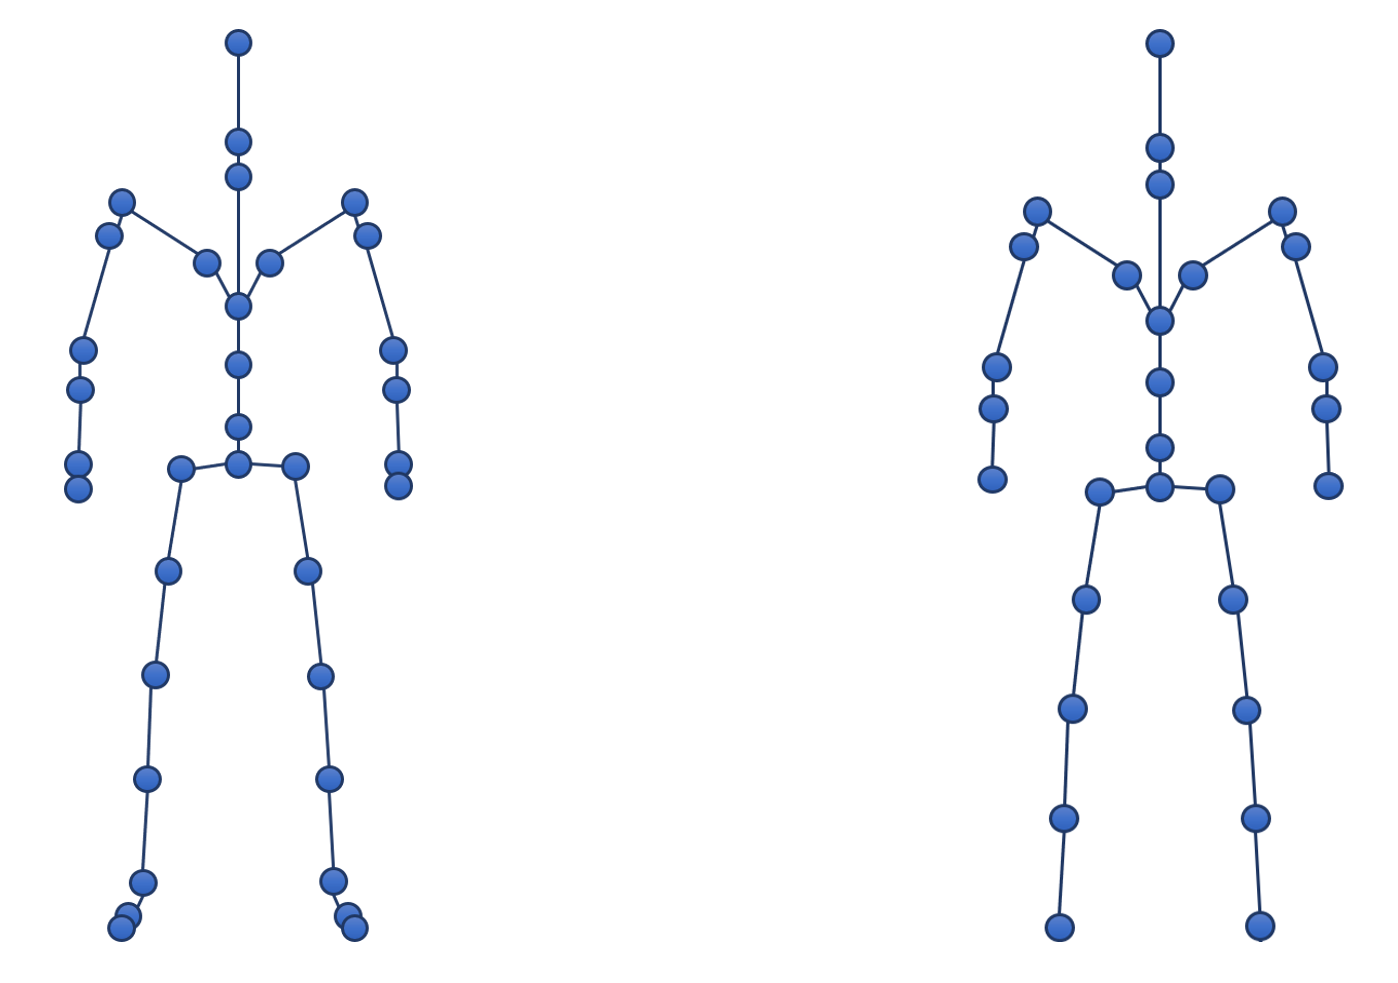
\includegraphics[height=130px]{images/implementation/mhad_skeletons.png}
  \caption[The skeleton structure used in MHAD dataset before and after modification.]{The original skeleton structure used in MHAD dataset ({\it left}) vs. the modified skeleton ({\it right}).}
  \label{fig:mhad_skeletons}
\end{center}
\end{figure}

\noindent 
As the real datasets do not comprise the partition into the particular body regions, the automated technique for the annotation has been proposed in the original implementation of PBPE model. Each skeletal joint is assigned one body region. Using the automatic annotation, each point of the point cloud is associated with the closest skeletal joint based on Euclidean distance. The example of the annotated point cloud is shown in Figure~\ref{fig:reg_annotation}.\par 

\vspace{5mm}
\begin{figure}[H]
\begin{center}
  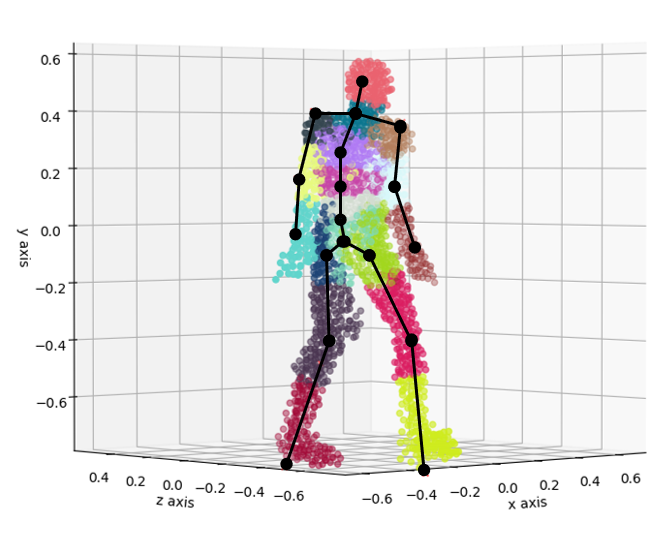
\includegraphics[height=200px]{images/implementation/region_annotation.png}
  \caption[The automatic body region annotation on real data.]{The automatic body region annotation on a sample real data point cloud.}
  \label{fig:reg_annotation}
\end{center}
\end{figure}

\subsubsection{Modifications}
For the sake of achieving as accurate pose estimation as possible, we made a number of modifications to the model implementation, to use the full potential of the selected framework. In the architecture of our modified PBPE model, we put even greater emphasis on the local feature extraction, chaining additional pseudo-convolutional layers into the shared MLP before max-pooling. Aside from that, we also left out the dropout in the regression branch, since with a help from the auxiliary branch, the model had not suffer from overfitting. Moreover, we skipped all the batch normalization layers in the main branch, since the performance improved when excluding them.\par
\vspace{5mm}
\noindent
The loss function has been replaced by mean absolute error, as it helped the model to converge faster in our case. The hyperparameters of the model mostly preserve the same values as in the original paper, except for the learning rate and loss weights. Given by our observations, we fine-tuned the weight parameter of the global loss to $w_g=1$, and decreased the weight of the segmentation branch to $w_a = 0.01$. We set the initial learning rate to $5^{-4}$, while reducing it with an exponential decay rate of $d = 0.2$ in each epoch. Again, the differences between the performance with the particular hyper-parameter values might be caused by switching to another deep learning framework. 


\section{Segmentation-Guided Pose Estimation} % TODO

This section is dedicated to the implementation of a novel approach we present as one of the contributions of this thesis. The core of the proposed method is a two-stage pipeline, consisting of a body segmentation network and a regression network. The two subsequent stages take a point cloud as an input and produce skeletal joint coordinates as a result.\par
\vspace{5mm}
\noindent The aim of the model is to embrace both local and global features of the input point cloud, and thus increase the accuracy of the final estimation of the human pose. Also, the model makes use of the residual connections in-between the layers to help the gradient flow, and to avoid the degradation problem as the network depth increases.


\subsubsection{Model structure}
In both networks of the pipeline, the input point clouds are being processed in the similar fashion as in the PBPE model, i.e. by employing the shared multi-layer perceptron modules. The architecture of the whole pipeline is described in Figure~\ref{fig:4chan_pipeline}.\par
\vspace{5mm}
\noindent 
As a first part of our pipeline, we propose a segmentation network with an architecture similar to the one of the regression model, instead of making use of one of the existing segmentation methods. While utilizing the same main modules in the segmentation and regression model, we believe preserving a similar network-specific representation of the body pose in both models works for the benefit of more accurate pose estimation.\par
\vspace{5mm}
\noindent In the first stage, the pre-processed point clouds are fed into the segmentation network, which performs a pointwise classification into the corresponding body regions. The architecture of the model, as shown in Figure~\ref{fig:4chan_pipeline}~(top), is based on the shared MLP modules. To obtain global features, the output vector of the first shared MLP is aggregated in a pooling layer across all points of the point cloud. Since the local information is essential in the task of semantic segmentation as well, we want to avoid losing the local context after the max pooling aggregation. Therefore, the local features extracted from the intermediate layers of the shared MLP are concatenated with the aggregated global features and sent off to the second shared MLP module. After the second shared MLP, the model outputs the predicted per-point classification probabilities for each body region.\par
\vspace{5mm}
\noindent In order to help the gradient flow, and enhance the feature propagation, we improved the shared MLP modules in our approach by adding residual connections in-between the convolutional layers. Referring to the figure, the numbers in the brackets near the shared MLP blocks describe the number of filters in the respective $1 \times 1$ convolutional layers.\par
\vspace{5mm}
\noindent Since the real data does not come with body-parts segmentation, we perform an automatic annotation of the point clouds to acquire ground truth body region classification of the data, in the same way as described in PBPE model implementation.\par

\vspace{5mm}
\begin{figure}[H]
\begin{center}
  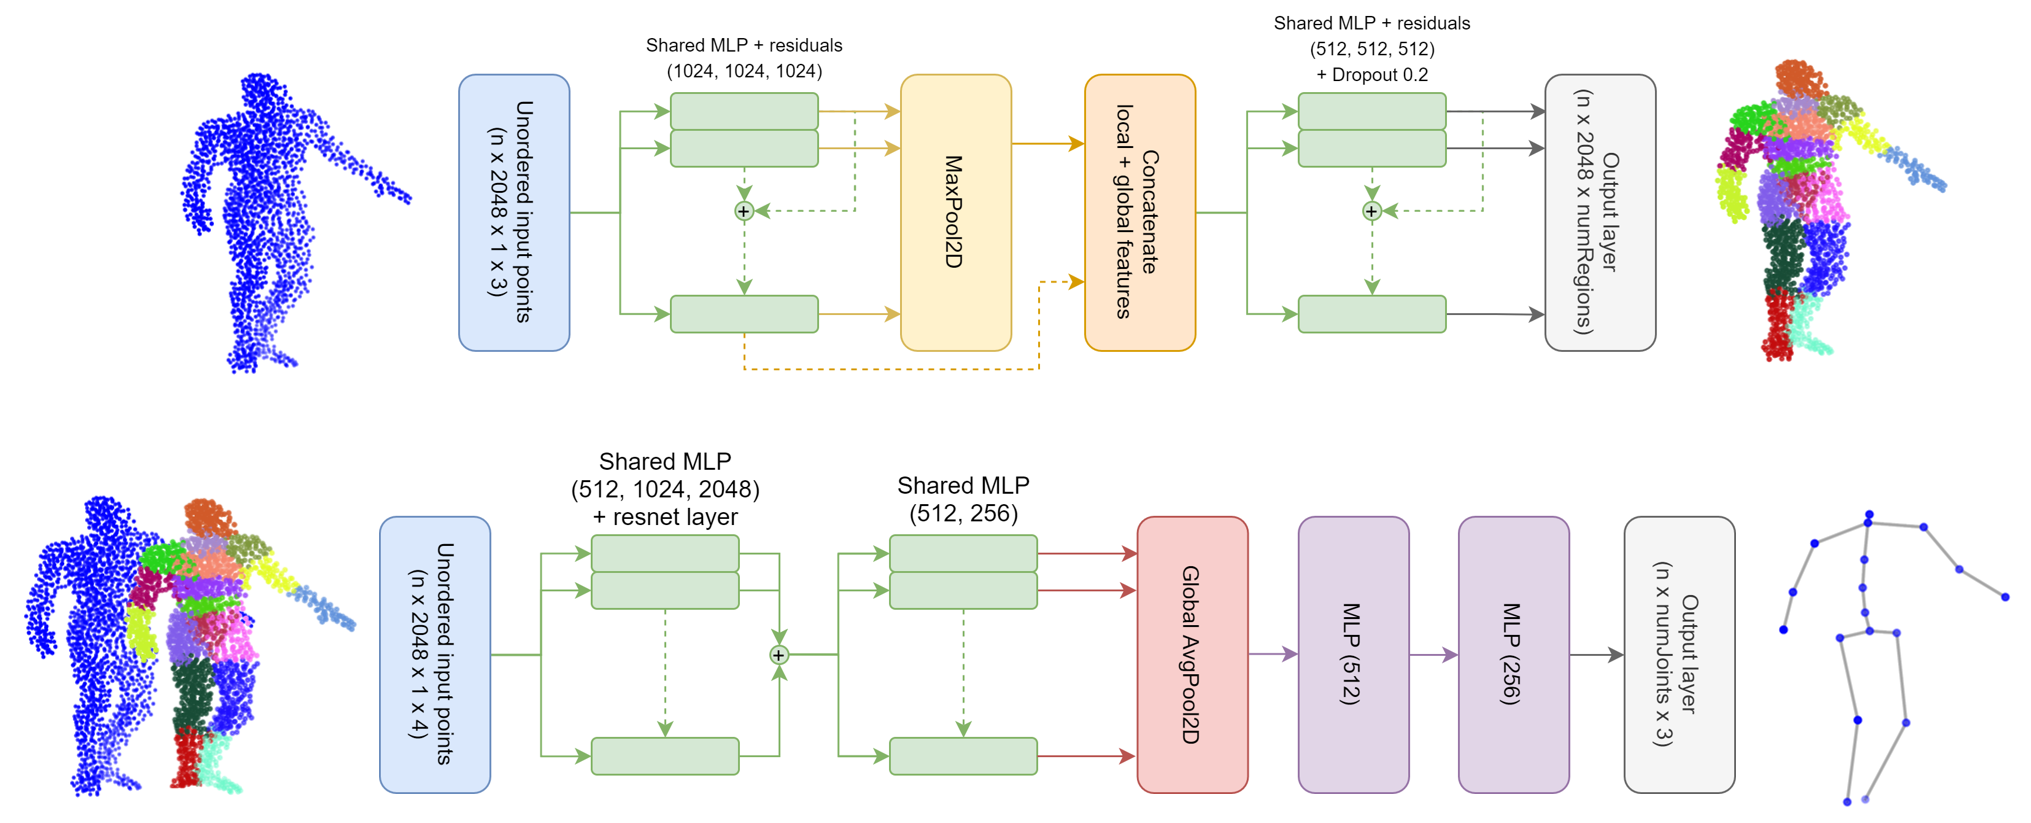
\includegraphics[width=\textwidth]{images/implementation/4chan_pipeline_mine2.png}
  \caption[The Segmentation-Guided Pose Estimation pipeline.]{ The Segmentation-Guided Pose Estimation pipeline: First, point clouds are segmented into body regions in the segmentation network ({\it top}), then the input point clouds are concatenated with the predicted per-point body region assignment as a fourth channel, and fed into the regression network ({\it bottom}).}
  \label{fig:4chan_pipeline}
\end{center}
\end{figure}

\noindent The second stage of our pipeline is based on the regression network. To incorporate the idea of retaining both local and global context of the input point clouds, the initial 3D point cloud is concatenated with the predicted pointwise region assignment after the body region segmentation, forming a four-channel input point cloud, which is passed to the regression model (as indicated in Figure~\ref{fig:4chan_pipeline}, bottom). Again, the network incorporates two shared MLP blocks. The first one contains three convolutional layers with $1 \times 1$ kernels, followed by one residual connection adding up the outputs of the three preceding layers. To control the number of parameters of the network, the second shared MLP includes two layers and no additional skip connections. To avoid having majority of the model parameters concentrated in the first fully-connected layer, the global average pooling is utilized instead of a simple flattening layer to spatially average across all points right before the fully-connected layers. As indicated in the figure, the pooling layer is followed by two dense layers with 512 and 256 filters, respectively. Finally, the model estimates the 3D skeletal joint coordinates of the captured human subject as the output.\par

% TODO in results ? - the 4chan model proved to benefit from the redundancy in the network inputs, being able to absorb the local and global context at once.

\subsubsection{Loss function}
In the first (segmentation) network, the categorical cross-entropy is employed as a loss function, to measure the accuracy of the body part classification. In the case of the regression network, the mean absolute error between the predicted locations and the ground truth labels of all skeletal joints is used to determine the model loss.

\subsubsection{Initialization}
Both networks are trained using the Adam optimizer with the initial learning rate equal to $10^{-3}$, and an exponential decay rate of $d=0.2$ applied at the end of each epoch. All weights are initialized with Xavier normal initializer. The batch size is fixed to $b=32$ for both models.

\subsubsection{Data pre-processing}
Prior to sending the input point cloud to the first neural network, the background scene is segmented out – the ground floor and the surrounding walls are removed using RANSAC plane fitting algorithm, and the biggest cluster of the point cloud is extracted, being considered the captured human subject. To unify the dimension of the model input, the point cloud is subsampled to a fixed number of points using the farthest point sampling. We set the hyperparameter determining the number of points in each point cloud to $p = 2048$, yielding a fair density of the input data. Both the ground truth skeleton coordinates, as well as the input point clouds, are normalized to the range $[-1, 1]$ along each axis, using minimum and maximum values of the whole training set.

